\section{pca2densitymap} \label{sec-pca2densitymap}

\subsection{General}

The \emph{pca2densiymap} tool allows you to visualize the the sequence density
in a pca file by generating a portable network graphics (PNG)
image. This basically 
generates a histogram by laying a rectangular grid across a projection
into two/three dimensional subspace, spun by principal components. The
tool then counts how many sequences are found within a square/cube
and attributes this value to a pixel/voxel in the final
image/images. The 3D version creates a stack of images. To overcome
the limitations of an image based tool such as this one,
one may refer to the \emph{pca2densityfile} tool outlined in section
\ref{sec-pca2densityfile}. 

\subsection{Usage}

The tool can be called like:
\lstset{language=bash,
  caption={Calling the \emph{pca2densitymap} tool},
  label=lst-pca2densitymap-call}
\begin{lstlisting}
pca2densitymap [fasta] [pca] [dimensions] [2D or 3D] \
  [invertal-length] [png-file-or-files]
\end{lstlisting}
and has the following arguments:
\begin{enumerate}
  \item \emph{fasta} The original FASTA file that has been transformed
    into a k-mer representation which was projected into a subspace
    spun by principal components. For instance by using the tools
    \emph{fasta2kmer} and \emph{kmer2pca} as described in sections
    \ref{sec-fasta2kmer} and \ref{sec-kmer2pca}.
  \item \emph{pca} A file containing the projections onto the
    principal components.
  \item \emph{dimensions} An integer describing how many dimensions
    the PCA subspace consists of.
  \item \emph{2D or 3D} Chose 2 for a 2-dimensional output or 3 for a
    3-dimensional output. 3-dimensional outputs are not fully tested
    though.
  \item \emph{interval-length} The grid spacing for our histogram.
  \item \emph{png-file-or-files} A path for the resulting PNG file. In
    case of a 3D output a whole stack of images with individual
    numbers for each slice our created.  
\end{enumerate}

\subsection{Example}
\lstset{language=bash,
  caption={Example of the \emph{pca2densitymap} tool},
  label=lst-pca2densitymap-example}
\begin{lstlisting}
pca2densitymap test.fasta test.pca 7 2 0.1 /temp/out.png
\end{lstlisting}
Here an image, \emph{out.png} will be generated that contains from
white ,most sequences per grid tile, to black, no sequences per grid
tile. As the image is 8 bits per pixel a range from 0 (black) to 255
(white) is available. Which might cause, due to the rescaling only a
few white points if the dataset contains very large peaks and
completely black background. \emph{test.fasta} is the sequence
dataset, \emph{test.pca} its projection into a 7 dimensional PCA
subspace. The tool always chooses only to treat either the first two or
three dimensions, for the 2D or 3D case respectively.
We generate a two dimensional output with a grid spacing of
0.1 [k-mer frequencies]. The tool yields some information about
the image generated:
\lstset{language={},
  caption={Text output of the \emph{pca2densitymap} tool},
  label=lst-pca2densitymap-txt-out}
\begin{lstlisting}
   shift x:  8.45373440
   shift y:  5.56738997
n points x:    122
n points y:     89
factor 255/maximum(intensity): 0.10814250
\end{lstlisting}
where shift x and y are origin of the image, in general on the upper
left. n Points x and y are the number of pixels according to the
spacing chosen that are calculated and stored in the output PNG
file. The last value is the scalefactor that has been used in order to
scale the the densities from 0 to 255 or from black to dark. A sample
of an image generated using this tool is highlighted in figure
\ref{fig-pca2densitymap}.
\begin{figure}
  \begin{center}
    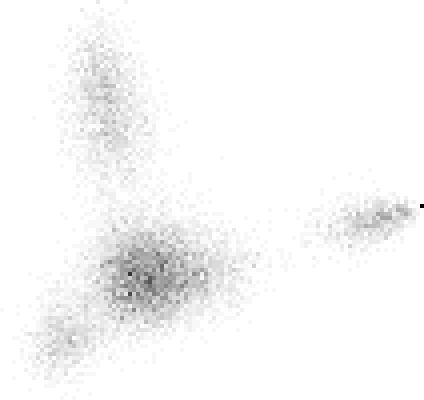
\includegraphics{pca-density.png}
    \caption{The sequence density in a two dimensional PCA subspace of
    a k-mer representation. The image was upscaled and color inverted
    for printing using the Gnu Image Manipulation Program (GIMP)
    \cite{gimp}.}
    \label{fig-pca2densitymap}
  \end{center}
\end{figure}

\subsection{Implementation}
The interface to this tool is implemented in \emph{pca2densitymap.c}.
The engine of the tool resides in \emph{density.c}.
